\documentclass[
	10pt,
	a4paper,
]{report}

% Random text
\usepackage{blindtext}
\usepackage{lipsum}

% Making fancy header and footers
\usepackage{fancyhdr}

% Danish letters
\usepackage[utf8]{inputenc}

% Reset footnote counter on new page
\usepackage[bottom, perpage]{footmisc}

% Math symbols
\usepackage{amssymb}

% For coloring \ref{}
\usepackage{hyperref}
\hypersetup{
	colorlinks,
	linkcolor={red!50!black},
	citecolor={blue!50!black},
	urlcolor={blue!80!black}
}

% Dots in Content
\usepackage{tocloft}

% Enable \todo{<task>}
\usepackage{todonotes}

% Adds Bibliography section to Contents
\usepackage[nottoc,notlof,notlot]{tocbibind}

% For Glossaries and addes them to Contents
\usepackage[toc]{glossaries}

% Insert PDF as page
\usepackage{pdfpages}

% For pretty tables
\usepackage{booktabs}
\usepackage{tabu}
\setlength{\tabcolsep}{10pt}
\renewcommand{\arraystretch}{1.2}

% Page margins
\usepackage{geometry}
\geometry{
	a4paper,
	left 	= 3cm,
	right 	= 3cm,
	top 	= 4cm,
	bottom 	= 4cm
}

% Enable \today
\usepackage{datetime}

% Enables \url{}
\usepackage{url}

% For translating document tag titles like 'Indholdsfortegnelse'
% instead of 'Contents', used below
\usepackage[english]{babel}
\addto\captionsenglish{\renewcommand{\contentsname}{Indholdsfortegnelse}}
\addto\captionsenglish{\renewcommand{\chaptername}{Kapitel}}
\addto\captionsenglish{\renewcommand{\bibname}{Litteraturliste}}
%\addto\captionsenglish{\renewcommand{\mtctitle}{Kapitel indhold}}

% For removing "Chapter X" from chapter headings
\usepackage{titlesec}
\titleformat{\chapter}{\huge\bf}{\thechapter.}{20pt}{\huge\bf}

% Increase rowspacing
\addtolength{\jot}{1em}

% Unknow packages
\usepackage[pages=some]{background}
\usepackage{subcaption}
\usepackage{nopageno}
\usepackage{graphicx}
\usepackage{lastpage}
\usepackage{caption}
\usepackage{amsmath}
\usepackage{wrapfig}
\usepackage{float}


\pagestyle{fancy}
\renewcommand{\headrulewidth}{1pt} % Header line thickness
\renewcommand{\footrulewidth}{0pt} % Footer line thickness
% Header 
\lhead{ITITS}   \chead{IT Sikkerhed - Disposition}     \rhead{\today}
% Footer 
\lfoot{}            \cfoot{}                    \rfoot{\thepage}

\begin{document}
    \pagenumbering{Roman}    
    % Titlepage

\newcommand{\myTitle}{Introduktion til IT-sikkerhed}

\title{\myTitle}
\date{}

\begin{titlepage}
	\begin{center}
		\bfseries{
		\huge UNIVERSITY OF AARHUS
		\vskip.2in
		\textsc{\LARGE Faculty of Science}
		\vskip.2in
		\large Department of Engineering
		\vskip1cm
		\huge \myTitle}
	\end{center}

	\vskip2cm

	\begin{figure}[H]
		\centering
		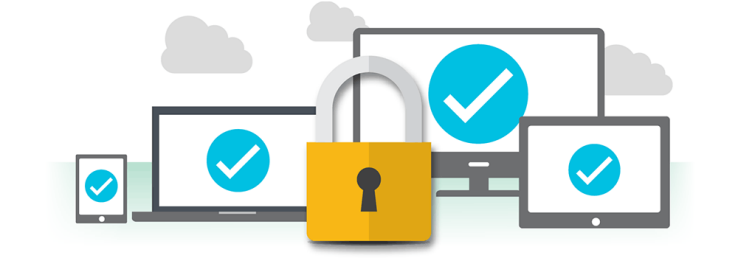
\includegraphics[width=0.9\linewidth]{figs/titlepagefig}
	\end{figure}

	\vskip2cm

	\begin{minipage}{.30\textwidth}
		\begin{center}
			\large
			Bjørn Nørgaard\\
			IKT\\
			201370248\\
			bjornnorgaard@post.au.dk
		\end{center}
	\end{minipage}
	\hskip.3\textwidth
	\begin{minipage}{.30\textwidth}
		\begin{center}
			\large
			Joachim Andersen\\
			IKT\\
			20137032\\
			joachimdam@post.au.dk
		\end{center}
	\end{minipage}

	\vskip4cm

	\centering
	\bfseries{
		\Large Sidste ændring: \today \ at \currenttime}

	\LaTeX-koden kan findes her:\\
		\url{www.github.com/bjornnorgaard/itits}
\end{titlepage}
    % Depth of Contents
\setcounter{tocdepth}{2}

% Links in text are red, but Contents links
% should remain black text.
\hypersetup{
	colorlinks,
	linkcolor={},
}

% Colors on links and refs
\hypersetup{
	colorlinks,
	linkcolor={black},
	citecolor={blue!50!black},
	urlcolor={blue!80!black}
}

% Comment this line before release
%\listoftodos

% Select list to display
\tableofcontents
%\listoffigures
%\lstlistoflistings
%\listoftables

% Removed pagenumbers from Contents
\thispagestyle{empty}

% Clears rest of page
\cleardoublepage

% Resets pagecounter after preamble
\setcounter{page}{1}

    \pagenumbering{arabic}

	% Chapter for testing
	%%% Beskrive de vigtigste begreber og værktøjer inden for kryptologi
\section{Kryptologi}

	% Chapters begin
	%% Beskrive de vigtigste begreber og værktøjer inden for kryptologi
\section{Kryptologi}\newpage
	
	%% Kendskab til sikkerhedsstandarder og lovgivning i relation til IT-sikkerhed
	%% Beskrive de vigtigste begreber og værktøjer inden for kryptologi
\section{Kryptologi}\newpage
	%% Beskrive de vigtigste begreber og værktøjer inden for kryptologi
\section{Kryptologi}\newpage
	
	%% Beskrive de vigtigste sikkerhedsrisici inden for sikre it-systemer,
	%% Beskrive de vigtigste begreber og værktøjer inden for kryptologi
\section{Kryptologi}\newpage
	
	%% Beskrive de vigtigste begreber og værktøjer inden for kryptologi
	%% Beskrive de vigtigste begreber og værktøjer inden for kryptologi
\section{Kryptologi}\newpage
	
	%% Anvende kodebiblioteker og værktøjer til at sikre fortrolighed, integritet og tilgængelighed af data
	%% Beskrive de vigtigste begreber og værktøjer inden for kryptologi
\section{Kryptologi}\newpage
	%% Beskrive de vigtigste begreber og værktøjer inden for kryptologi
\section{Kryptologi}\newpage
	%% Beskrive de vigtigste begreber og værktøjer inden for kryptologi
\section{Kryptologi}\newpage
	%% Beskrive de vigtigste begreber og værktøjer inden for kryptologi
\section{Kryptologi}\newpage
	
	%% Analysere konkrete brugsscenarier og identificere de vigtigste sikkerhedsrisici
	%% Beskrive de vigtigste begreber og værktøjer inden for kryptologi
\section{Kryptologi}\newpage
	%% Beskrive de vigtigste begreber og værktøjer inden for kryptologi
\section{Kryptologi}\newpage
	
	%% Sammenligne og evaluere forskellige begreber og teknikkers anvendelighed til løsning af konkrete sikkerhedsproblemer
	%% Beskrive de vigtigste begreber og værktøjer inden for kryptologi
\section{Kryptologi}\newpage
	% Chapters end	
\end{document}
